
\section{Introduction/Motivation}

\quad Yelp is a website which allows users to create an account and review businesses. Our goal is to analyze data from Yelp to gain further insight for business owners to develop a satisfactory experience for their customers. Yelp has a public dataset available on their website with information about users, businesses, and reviews.

\quad Our  rst objective is to determine if certain attributes are indica- tive of business success. If we can find a way to predict whether or not a business will do well later on in its operation, that information will be useful to businesses looking to improve their model.

\quad Our second objective is to analyze the text of reviews for a sen- timent. The sentiment analysis will show the emotions conveyed by the reviewer as being pleased or angry at their experience with the business. Using the results of this analysis we hope to be able to determine if certain times of day, city locations, or other factors contribute to the experience of a customer. This information could also contribute to a business model. As an example, if certain loca- tions are more prone to angry customers it could indicate that the people in that area have high standards, the businesses are poorly run, or just that those customers tend to leave angry reviews.

\quad Our last objective is to  nd recurring problems in businesses. We will analyze review text to  nd the speci c issues that people are having with businesses. If a business has many reviews which all indicate a similar issue, then that is something a business owner would want to be aware of so that they can eliminate the problem.

% Head 1
\section{Prior Work}

Since our problem involves predictions surrounding businesses, we sought out similar research to guide our investigation. Thus, we focus our literature review on studies that utilized some form of sentiment analysis, constructed predictive models, and/or conducted meta-analysis of trends in the aforementioned sentiment, rating, or business interest.

% Head 2
\subsection{Predicting Business Attention}

A previous winner, Hood et al., published a paper on assessing a business?s current rating/review state and future expectations with respect to review numbers on Yelp. The bulk of their work centered around the creation of additional features for the data (e.g. number of similar businesses within 1km, features of subsets of reviews such as average rating and number of unique users). From there they utilized various feature reduction and clustering techniques to build a prediction model. They were able to identify features that o ered greater accuracy in prediction of interest in the business (calculated as the predicted number of reviews within 6 months after a target date) as well as a create model for prediction that outperformed a basic linear regression.

% Head 3
\subsection{Latent Subtopics}

Huang et al. (2013) utilized probabilistic models to discover under- lying subtopics within Yelp reviews. This o ered a framework to categorize the reviews based on review text. From here, they were able to analyze the prevalence of various star ratings within each category. In this way, they could advise business owners as to the common trends among good and bad reviews that may not be ap- parent without considering the review text. McAuley and Leskovec built on this idea by combining such latent review topics with hidden rating driving factors, allowing them construct a rating prediction model.

\subsection{Reviews and Revenue}

In one of the more in uential papers on the subject, Michael Luca showed a correlation between Yelp rating and revenue, highlighting the fact that rounding to half stars could signi cantly impact two similarly-rated restaurants if their averages fell on either side of the divide (e.g. 3.24 and 3.26). He goes on to build a model of market response based on review volume as well as the impact of user expertise. He concluded that such responses are consistent with a Bayesian learning model.

\section{Proposed Work and Dataset Information}

\subsection{Proposed Work}

The dataset has many optional attributes. There is an attribute called 'attributes' that is a list of optional attributes. The dataset is inconsistent and cannot be relied upon for each business. For instance, one of these attributes is ?Bike Parking?. This attribute is either true, false, or nonexistent. Speci cally the fact that this attribute might not be available for multiple businesses makes it unreliable.

\quad In addition, the data is not only restaurants but any kind of busi- ness. As a result they have another piece of data which is the cat- egories list. For each business this attribute attempts to classify the business. However some categories are extremely broad and the same type of business can be described in di erent ways. One example is that there is a bakery, but it?s also categorized as food. Many businesses will sell food, but the category of food will not be in their list of categories and instead it will be  lled with more speci c categories like Italian food.

\quad The majority of the data cleaning process will be involved in handling missing data. It is possible to  ll in these missing values with default values like false but this can be dangerous to make assumptions about what businesses have and don?t have.

\quad The Yelp dataset contains up to one million di erent attributes about businesses from 11 di erent cities in 4 countries. The majority of these attributes will be unnecessary so there will be a large e ort in data reduction. For instance there are photographs included, but our questions does not require image analysis. There also attributes such as postal codes that are unnecessary because latitude and longitude is more accurate.

\subsection{Dataset}

The Yelp dataset comes from the Yelp Dataset Challenge. This is an ongoing challenge and this is the ninth round. The challenge offers \$5,000 to the winner and the  final submission is an academic paper.

\quad We will be considering the following from the Yelp dataset:

\begin{itemize}
	\item{4.1 million reviews}
	\begin{verbatim}
	"review_id":(encrypted review id),
	"user_id":(encrypted user id),
	"business_id":(encrypted business id)"
	"stars":(star rating, rounded to half-stars),
	"date":(date, formatted: YYYY-MM-DD),
	"text":"review text",
	"useful":('useful' vote count),
	"funny":('funny' vote count),
	"cool": ('cool' vote count),
	"type": "review"
	\end{verbatim}
	\item{Informationon144,000businessesin11citiesfrom4coun- tries (incl. the US, Germany, Canada, and the U.K. (with 1.1 million business attributes)}
	\begin{verbatim}
	"business_id":(encrypted business id),
	"name":"business name",
	"neighborhood": "hood name",
	"address":"full address",
	"city":"city",
	"state":"state"(if applicable),
	"postal code":"postal code",
	"latitude":latitude,
	"longitude":longitude,
	"stars":(star rating, rounded to half-stars),
	"review_count":(number of reviews),
	"is_open":0/1 (closed/open),
	"attributes":[(localized attribute tags)],
	"categories":[(localized category names)],
	"hours":[(hours strings)],
	"type": "business"
	\end{verbatim}
	\item{Over 1M users}
	\begin{verbatim}
	"user_id":(encrypted user id),
	"name":"first name",
	"review_count":(number of reviews),
	"yelping_since": (date, formatted: YYYY-MM-DD),
	"friends":[(encrypted user ids)],
	"useful":('useful' vote count sent by user),
	"funny":('funny' vote count sent by user),
	"cool": ('cool' vote count sent by user),
	"fans":"number of fans the user has",
	"elite":["an array of years the user was elite"],
	"average_stars":floating point average like 4.31,
	"compliment_type": (compliment count),
		...(same for each compliment type)...
	"type":"user"
	\end{verbatim}
	\item{Over 200,000 user-submitted photographs, 947,000 tips, and aggregated check-in data}
\end{itemize}

\section{Methods and Tools}

\quad The tools and methods used for this project will include a database for storing and integrating the data, libraries and modules for cleaning and preprocessing, and various tools for transformation, mining, pattern evaluation, and knowledge presentation. Given the json-formatted data, we've opted for using a NoSQL database like MongoDB or Cassandra. Fortunately, there are a number of options, considering our educational status, that will allow large storage volume as well as low latency read/write access. Hosting in such a manner will requireA number of Python libraries like Dora and FTFY (?fixes text for you?) intended for data cleaning and preprocessing will be used for these purposes. Yelp has already performed a substantial amount of cleaning on the data, so it is likely that minimal additional cleaning will be necessary, save for replacing missing values as mentioned above.

\quad Numpy and Scipy will be used to transform and mine the data, and other Python modules like Seaborn and Plotly (a Python API for D3) will be used for knowledge visualization and presentation. Finding angry reviews and recurring problems will make heavy use of NLP, so the team will rely on tools like Weka, the Text Analytics API from Microsoft Cognitive Services, and possibly some custom supervised text classi ers trained with the Facebook fastText pretrained word vectors to perform sentiment analysis on the review text.


\section{Evaluation}

\subsection{Methodology}

\quad Evaluating our predictions as to whether a business success will hinge on comparing the star rating (from one to  ve stars) and our predicted star rating based on the other attributes in the review, such as day of the week and month, season, or location. This could be done by training an ML algorithm like Kernel Ridge regression on 80\% of the data and testing it on the remaining 20\%, and then adjusting parameters to minimize the error between the actual star ratings and our predicted star ratings for the testing data.

\quad Evaluating the sentiment analysis of the review text will likely be simple given that we will be using tools like Weka and Microsoft Sentiment Analysis (see following section) to perform sentiment analysis rather than creating entirely custom algorithms. These tools incorporate helpful metrics to analyze the error of a particular output. Alternatively, we can manually verify the sentiment of a (relatively small) number of reviews by reading them and comparing our human judgements of the sentiment to the output of the tools. For evaluating recurring problems, we will employ a similar approach, except we will group reviews by business and analyze them as a time series to and recurring issues.

\quad For all three of the objective questions, employing association rule frameworks that use support-confidence frameworks will be helpful to and strong associations, while null-invariant measures like the Kulczynski measure or the cosine measure will be helpful to determine how interesting these associations are.

\section{Progress}

\quad Our most significant hurdle was in getting our data into a tool for some initial experimentation. While JSON formatting is extremely common in web applications, it seems that it's integration in data mining software has lagged. After several unsuccessful attempts to view our data through WEKA, we opted for a different tool, RapidMiner. From here, we've taken two routes: 1) running a python script to convert the JSON to CSV and 2) import the data into a local MongoDB instance and connect via the proper port. Both methods have finally allowed some degree of visualization to better direct our inquiry.

\section{Results}

\subsection{Businesses}

\quad After importing the CSV formatted version of the data we tested some basic visualization of the data. For instance, in Figure 1 we created a histogram of the average star for a business versus the state in which it?s located. Basic graphs like these help refine our question. For example, why does Illinois have significantly lower average stars than others? 

\quad The most pervasive issue with our business data is that many entries are missing data, most notably the 'attributes' and address information. Since attributes are managed by the account owner, they vary widely across the businesses.

\begin{figure}
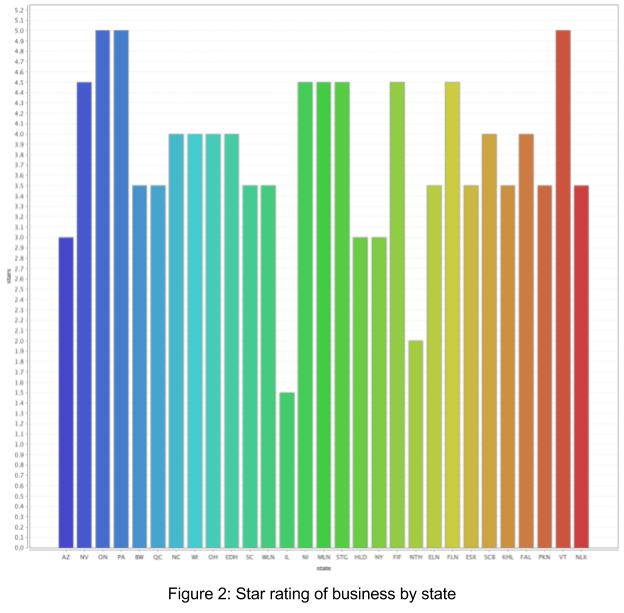
\includegraphics[width=0.75\textwidth, center]{b_rating_by_state}
\end{figure}

\subsection{Users}

\begin{figure}
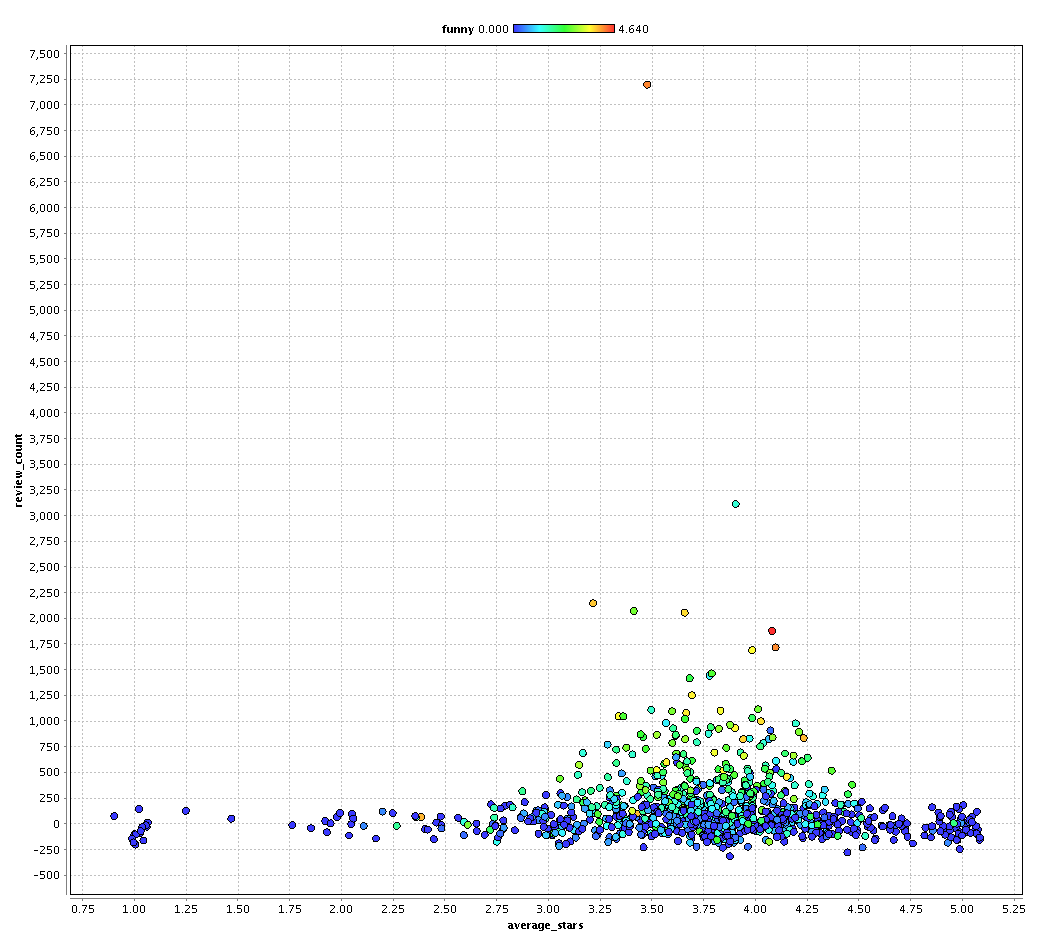
\includegraphics[width=0.5\textwidth, center]{u_reviews_vs_stars}
\end{figure}

\quad
\section{Next Steps}

\quad Some major milestones before Spring Break (March 27th) will include organizing and integrating all the data in a relational database, as well as cleaning and preprocessing the data. After these steps have been completed, it will be much easier to begin preliminary investigations into our main questions for the project, such as reducing the entire set of attributes into just those that will be mined for each question. Milestones after Spring Break prior to April 11th will include using the tools listed above to answer two of our objective questions, while work after that will focus on answering the remaining question and writing the final report.

% Start of "Sample References" section

%\section{Typical references in new ACM Reference Format}
%A paginated journal article \cite{Abril07}, an enumerated
%journal article \cite{Cohen07}, a reference to an entire issue \cite{JCohen96},
%a monograph (whole book) \cite{Kosiur01}, a monograph/whole book in a series (see 2a in spec. document)
%\cite{Harel79}, a divisible-book such as an anthology or compilation \cite{Editor00}
%followed by the same example, however we only output the series if the volume number is given
%\cite{Editor00a} (so Editor00a's series should NOT be present since it has no vol. no.),
%a chapter in a divisible book \cite{Spector90}, a chapter in a divisible book
%in a series \cite{Douglass98}, a multi-volume work as book \cite{Knuth97},
%an article in a proceedings (of a conference, symposium, workshop for example)
%(paginated proceedings article) \cite{Andler79}, a proceedings article
%with all possible elements \cite{Smith10}, an example of an enumerated
%proceedings article \cite{VanGundy07},
%an informally published work \cite{Harel78}, a doctoral dissertation \cite{Clarkson85},
%a master's thesis: \cite{anisi03}, an online document / world wide web
%resource \cite{Thornburg01, Ablamowicz07, Poker06}, a video game (Case 1) \cite{Obama08} and (Case 2) \cite{Novak03}
%and \cite{Lee05} and (Case 3) a patent \cite{JoeScientist001},
%work accepted for publication \cite{rous08}, 'YYYYb'-test for prolific author
%\cite{SaeediMEJ10} and \cite{SaeediJETC10}. Other cites might contain
%'duplicate' DOI and URLs (some SIAM articles) \cite{Kirschmer:2010:AEI:1958016.1958018}.
%Boris / Barbara Beeton: multi-volume works as books
%\cite{MR781536} and \cite{MR781537}.
%
%A couple of citations with DOIs: \cite{2004:ITE:1009386.1010128,
%  Kirschmer:2010:AEI:1958016.1958018}. 

% Bibliography
\bibliographystyle{ACM-Reference-Format}
\bibliography{sample-bibliography}
